\documentclass[handout]{beamer}

\title{Content Security Policy \& Other Web Security Headers}
\author{David Fischer}
\date{November 18, 2021}

%% Beamer Themes
\usetheme{Berlin}
\usecolortheme{dove}
\usefonttheme{serif}

%% Packages
% Pygments must be accessible to use minted and --shell-escape
%  must be used with pdflatex
\usepackage{minted}
\usepackage{hyperref}
\usepackage{amssymb}
\usepackage[font=scriptsize,labelformat=empty]{caption}


\setbeamertemplate{footline}{
  \hspace*{.2cm}
  \scriptsize{
    \insertshorttitle
    \hspace*{50pt}
    \hfill
    \insertframenumber/\inserttotalframenumber
    \hspace*{.2cm}
  }
  \vspace{9pt}
}


%% Page 2: Title screen
%
%  Modern browsers like Firefox, Chrome, Edge, and Safari
%  include a lot of new security features to help keep you safe while browsing the web.
%  However, in order to keep backwards compatibility, a lot of these are opt-in features.
%  They allow site operators to tell the browser that their site has these safety features
%  and the browser will respect them and apply them to keep you safe.
%  While there's a lot of newer features from new cookie attributes to subresource integrity,
%  I'm going to talk about the optional features that are in HTTP headers.


%% Page 3: What is CSP
%
%  Of all the HTTP headers I'm going to talk about, content security policy
%  is the most complicated and the hardest to roll out properly to a large existing site.
%  It allows a web site operator to tell the browser what resources the browser should use on this site.
%  As an operator, if you know none of the forms on your site submit to any domain other than yours,
%  you can set CSP to prevent forms from being submitted to any other domain.
%  If you ever add such a form though, your header has to be changed.
%  This can be used to prevent whole classes of website attacks.


%% Page 4: Screenshot
%
%  This is an example of what happens when the browser violates CSP.
%  It's hard to get a complex policy right the first time,
%  but CSP can be rolled out bit by bit.
%  There's also a way to have the browser send violations to a specific URL
%  so they can be fixed.


%% Page 5: CSP in Django
%
%  This is just an example of a CSP setup in Django
%  It blocks mixed content (serving HTTP resources when the page is HTTPS)
%  and upgrades HTTP requests to HTTPS.
%  There's also a way to protect your own scripts (similar but different from Subresource Integrity).


%% Page 6: Strict Transport Security
%
%  Strict Transport Security prevents your site from being loaded over plain HTTP
%  (requiring HTTPS) after the first time a browser loads it.
%  All subsequent requests will go to HTTPS.
%  This can prevent insecure cookies from leaking
%  or other sensitive data from leaking. This is especially important
%  when accessing a site over an insecure network like public WiFi.
%  The browser will go directly to HTTPS for a certain amount of time (typically a year)
%  before checking again.
%  Django has support for this header out of the box.


%% Page 7: X-Frame-Options
%
%  This is an optional header to prevent a site from being iframed or framed.
%  If an attacker can trick a user to visit a framed site, they can exfiltrate
%  data while making their site look exactly like the original.
%  As a website owner, if you don't frame your site (and most sites don't)
%  it's easy to set this header.


%% Page 8: X-Content-Type-Options
%
%  Content type options is an important header to set for any site
%  that handles and serves user-uploaded content.
%  


%% Page 9: X-XSS-Protection
%
%  This header protects against some "reflective" XSS attacks.
%  Reflective XSS attacks are attacks where contents of the URL or query parameters (stuff after a ? in a URL)
%  are reflected back to the user on the webpage.
%  This header doesn't catch everything but it can add a second layer of protection
%  on top of app hardening.


%% Page 10: Referrer-Policy
%
%  The referrer policy header controls what is sent to sites on outbound links.
%  Any website with sensitive information in the URL should be interested in this header.
%  Django added the ability to control this header in 3.0.


%% Page 11: Additional headers
%
%  There's a few additional headers that most sites don't need yet.
%  I'm not going to talk a lot about them other than to mention that they exist.
%  The Permissions-Policy header got a little bit of notoriety earlier this year
%  as it could be used to disable Google's in-browser machine-learning to target Chrome users with better ads (FLOC).


%% Page 12: Mozilla Observatory
%
%  There's a lot to get right on these headers.
%  Mozilla Observatory is a website scanner that can help ensure the website configures these headers correctly.
%  The grades aren't the be-all-end-all in terms of web security,
%  but a higher grade usually signifies that a site takes security seriously.


\begin{document}

\maketitle

\begin{frame}
\frametitle{}
  {\huge Content Security Policy \& Other Web Security Headers}
\end{frame}


\begin{frame}
  \frametitle{What is Content Security Policy (CSP)?}
  \begin{itemize}
    \item An HTTP header (`Content-Security-Policy:')
    \item Allows the server to control what the browser can do
    \item For example, can prevent browsers that understand CSP from interpreting inline scripts, styles, or prevent forms from submitting to unauthorized domains
    \item When used appropriately, helps prevent many types of web security vulnerabilities (eg. XSS)
    \item Used extensively by GitHub, DuckDuckGo, Google, and other security conscious companies
  \end{itemize}
\end{frame}


\begin{frame}
  \begin{figure}[p]
    \centering
    \fbox{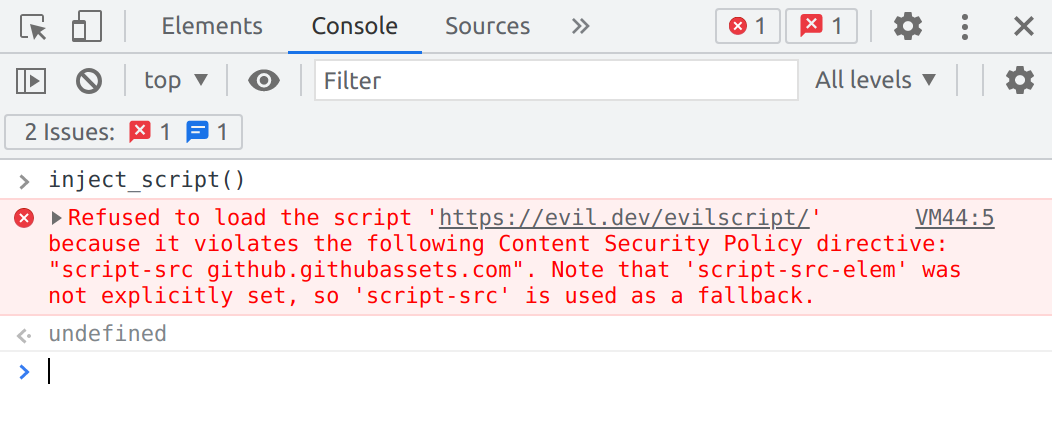
\includegraphics[height=0.4\paperheight]{includes/csp-blocking.png}}
    \caption{A blocked script from an untrusted domain}
  \end{figure}
\end{frame}


\begin{frame}[fragile]
\frametitle{CSP (with django-csp)}
{\tiny
\begin{minted}{python}
## settings.py

# https://django-csp.readthedocs.io/
MIDDLEWARE = (
    # ...
    'csp.middleware.CSPMiddleware',
)

# Block mixed content (HTTPS pages serve HTTPS resources)
# Upgrade plain HTTP requests to HTTPS
CSP_UPGRADE_INSECURE_REQUESTS = not DEBUG
CSP_BLOCK_ALL_MIXED_CONTENT = not DEBUG

# Don't allow iframing: Essentially the same as X-Frame-Options: Deny
CSP_FRAME_ANCESTORS = ("'none'",)

# These require a bit more finesse
# Includes a nonce (random single use string)
# <script nonce="{{request.csp_nonce}}"></script>
CSP_INCLUDE_NONCE_IN = ('script-src', 'style-src')

# Restrict the destination of various tags (img, form, etc.)
CSP_BASE_URI = CSP_CONNECT_SRC = CSP_FONT_SRC = ("'self'",)
CSP_IMG_SRC = CSP_FORM_ACTION = ("'self'",)
CSP_DEFAULT_SRC = ("'none'",)

# The admin is not currently CSP-friendly
CSP_EXCLUDE_URL_PREFIXES = ["/admin",]

\end{minted}
}
\end{frame}


\begin{frame}[fragile]
\frametitle{Strict-Transport-Security}
{\tiny

Strict Transport Security (HSTS) instructs a browser to always load a website over HTTPS, never HTTPS.
Even if you type http://duckduckgo.com into your browser, you'll go directly to https://duckduckgo.com.

\vfill

\begin{minted}{python}

## settings.py

# This middleware is installed by default in a new project
MIDDLEWARE = [
    'django.middleware.security.SecurityMiddleware',
    # ...
]

if not DEBUG:
    # Expire HSTS (reload the domain once over HTTP) after this many seconds
    SECURE_HSTS_SECONDS = 60 * 60 * 24 * 365

    # Don't load subdomains over plain HTTP either
    SECURE_HSTS_INCLUDE_SUBDOMAINS = True

    # With this setting, this site can be submitted to a preload list.
    # Browsers (Firefox, Chrome, Edge, Safari) ship with this list
    # and will never load any domain on it over plain HTTP
    SECURE_HSTS_PRELOAD = True

\end{minted}
}
\end{frame}


\begin{frame}[fragile]
\frametitle{X-Frame-Options}
{\tiny

The X-Frame-Options header allows controlling how a site can be framed (using `iframe' or `frame').
Framing is potentially dangerous as an attacker can frame a trusted site but detect or control inputs.
This is known as ``Clickjacking".

\vfill

\begin{minted}{python}

## settings.py

MIDDLEWARE = [
    # ...
    'django.middleware.clickjacking.XFrameOptionsMiddleware',
]

# My site should never be inside a frame
X_FRAME_OPTIONS = 'DENY'

# My site is allowed to frame itself
# X_FRAME_OPTIONS = 'SAMEORIGIN'

\end{minted}
}
\end{frame}


\begin{frame}[fragile]
\frametitle{X-Content-Type-Options}
{\tiny

Some browsers attempt to detect the content type of a file if it isn't specified.
For web apps that serve user-uploaded files, they can be crafted to trick this detection
and perhaps execute one type of file because the server thinks it is a different type.

\vfill

\begin{minted}{python}

## settings.py


MIDDLEWARE = [
    'django.middleware.security.SecurityMiddleware',
    # ...
]

# Browsers shouldn't try to detect content types (mime-types)
SECURE_CONTENT_TYPE_NOSNIFF = True

\end{minted}
}
\end{frame}


\begin{frame}[fragile]
\frametitle{X-XSS-Protection}
{\tiny

This header attempts to block some simpler XSS attacks.
If the browser detects some HTML tags or JavaScript in the URL parameters
and then sees the same content in the body, it will be blocked.
This helps, but won't protect against many other types of XSS attacks.

\vfill

\begin{minted}{python}

## settings.py


MIDDLEWARE = [
    'django.middleware.security.SecurityMiddleware',
    # ...
]

# Attempts to block some simple XSS attacks
# Applies the header "X-XSS-Protection: 1; mode=block"
SECURE_BROWSER_XSS_FILTER = True

\end{minted}
}
\end{frame}


\begin{frame}[fragile]
\frametitle{Referrer-Policy}
{\tiny

When a user clicks a hyperlink in their browser (but not when they type a URL or follow a bookmark),
the browser sends the URL of the referring page.
On some frameworks, this can leak keys or tokens from the URL.
There are some privacy considerations with this as well.

\vfill

\begin{minted}{python}

## settings.py


MIDDLEWARE = [
    'django.middleware.security.SecurityMiddleware',
    # ...
]

# Introduced in Django 3.0
# "same-origin" - only send the referrer on requests to the same origin (same server)
# "strict-origin" - send only the domain (example.com) to the referred site, not the full URL
# "strict-origin-when-cross-origin" - send the full URL but only to the same origin
#                                     for different origins, send just the domain
SECURE_REFERRER_POLICY = 'same-origin'

\end{minted}
}
\end{frame}


\begin{frame}
  \frametitle{Additional headers}
  \begin{itemize}
    \item \textbf{Public-Key-Pins - } Restrict the allowed root certificate authority (CA) used for HTTPS. Modern browsers trust a few thousand CAs by default. This can restrict that to a handful.
    \item \textbf{Feature/Permissions-Policy - } This feature is in early stages and isn't fully implemented. The name is even changing. However, this header restricts the allowed browser APIs. For example, if a site doesn't use geolocation or the accelerometer APIs, they can be disabled. If the site is ever compromised, the attacker will have fewer things they can do.
  \end{itemize}
\end{frame}


\begin{frame}
  \begin{figure}[p]
    \centering
    \fbox{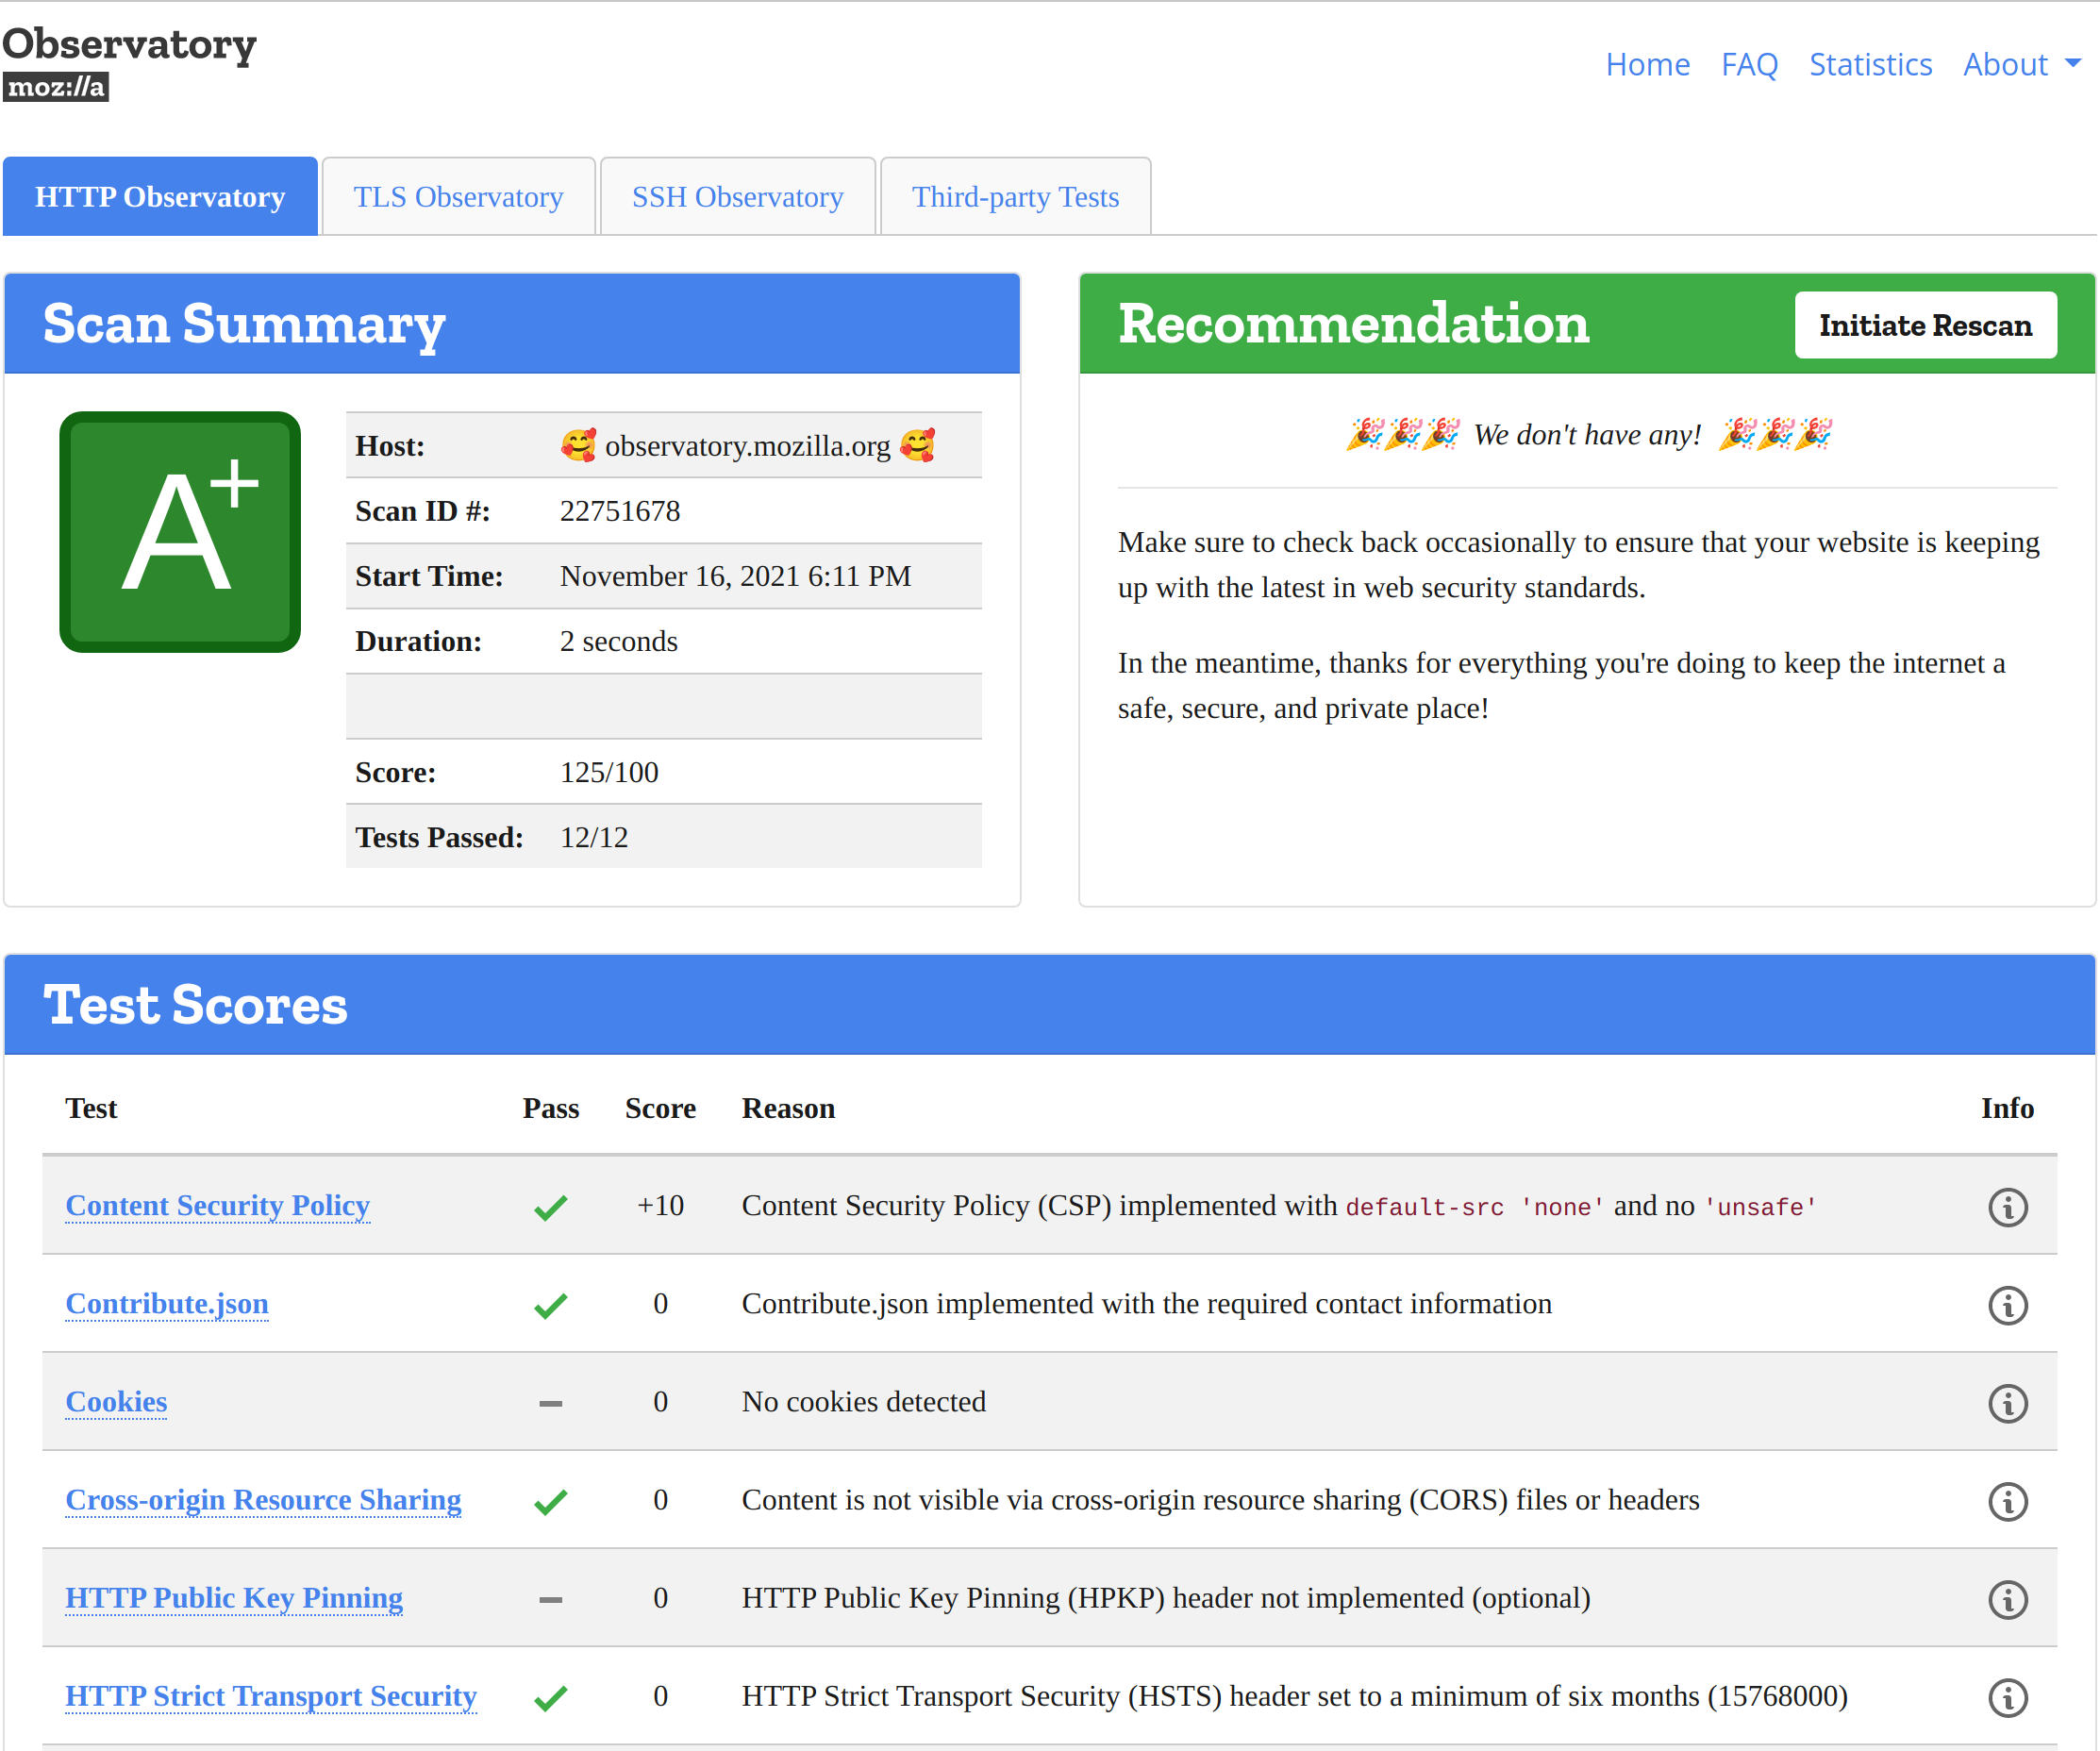
\includegraphics[height=0.7\paperheight]{includes/mozilla-observatory.png}}
    \caption{High score on Mozilla Observatory, a security scanner}
  \end{figure}
\end{frame}


\begin{frame}
\frametitle{Resources}
  \begin{itemize}
    \item {\small Mozilla Observatory: \href{https://observatory.mozilla.org/}{observatory.mozilla.org}}
    \item {\small CSP Evaluator: \href{https://csp-evaluator.withgoogle.com/}{csp-evaluator.withgoogle.com}}
    \item {\small SSL Labs: \href{https://www.ssllabs.com/}{ssllabs.com}}
    \item {\small CSP on MDN: \href{https://developer.mozilla.org/en-US/docs/Web/HTTP/CSP}{developer.mozilla.org}}
    \item {\small Django SecurityMiddleware: \href{https://docs.djangoproject.com/en/3.2/ref/middleware/\#module-django.middleware.security}{docs.djangoproject.com}}
  \end{itemize}
\end{frame}


\end{document}
